% Copyright 2004 by Till Tantau <tantau@users.sourceforge.net>.
%
% In principle, this file can be redistributed and/or modified under
% the terms of the GNU Public License, version 2.
%
% However, this file is supposed to be a template to be modified
% for your own needs. For this reason, if you use this file as a
% template and not specifically distribute it as part of a another
% package/program, I grant the extra permission to freely copy and
% modify this file as you see fit and even to delete this copyright
% notice. 

\documentclass[aspectratio=169]{beamer}
%\documentclass{beamer}

\setbeamersize{text margin left=5mm, text margin right=5mm}


\defbeamertemplate{headline}{my header}{%
\vskip1pt%
\makebox[0pt][l]{\,\insertshortauthor}%
\hspace*{\fill}\insertshorttitle/\insertshortsubtitle\hspace*{\fill}%
\llap{\insertpagenumber/\insertpresentationendpage\,}
}
\setbeamertemplate{headline}[my header]

\let\olditem\item
\renewcommand{\item}{\setlength{\itemsep}{\fill}\olditem}

\usepackage{soul}
\usepackage{tkz-euclide}
\usetikzlibrary{calc}
\usepackage[]{algorithm2e}
\usepackage{changepage}
\usepackage{amssymb}
\usepackage{xcolor}
\usepackage{mathtools}
\usepackage{tcolorbox}
\usepackage{tikz}
\usepackage{tikz-3dplot}
\usepackage[export]{adjustbox}
\usepackage{tabu}

% \usepackage[math]{cellspace}
% \cellspacetoplimit 4pt
% \cellspacebottomlimit 4pt
%\usetikzlibrary{arrows.meta}

%\setbeamertemplate{itemize items}{-}

%\usepackage{helvet}
\usefonttheme{professionalfonts} % using non standard fonts for beamer
%\usefonttheme{serif} % default family is serif
%\usepackage{fontspec}
%\setmainfont{Liberation Serif}

% There are many different themes available for Beamer. A comprehensive
% list with examples is given here:
% http://deic.uab.es/~iblanes/beamer_gallery/index_by_theme.html
% You can uncomment the themes below if you would like to use a different
% one:
%\usetheme{AnnArbor}
%\usetheme{Antibes}
%\usetheme{Bergen}
%\usetheme{Berkeley}
%\usetheme{Berlin}
%\usetheme{Boadilla}
%\usetheme{boxes}
%\usetheme{CambridgeUS}
%\usetheme{Copenhagen}
%\usetheme{Darmstadt}
%\usetheme{default}
%\usetheme{Frankfurt}
%\usetheme{Goettingen}
%\usetheme{Hannover}
%\usetheme{Ilmenau}
%\usetheme{JuanLesPins}
%\usetheme{Luebeck}
%\usetheme{Madrid}
%\usetheme{Malmoe}
%\usetheme{Marburg}
%\usetheme{Montpellier}
%\usetheme{PaloAlto}
%\usetheme{Pittsburgh}
%\usetheme{Rochester}
%\usetheme{Singapore}
%\usetheme{Szeged}
%\usetheme{Warsaw}


\def\mf{\ensuremath\mathbf}
\def\mb{\ensuremath\mathbb}
\def\mc{\ensuremath\mathcal}
\def\lp{\ensuremath\left(}
\def\rp{\ensuremath\right)}
\def\lv{\ensuremath\left\lvert}
\def\rv{\ensuremath\right\rvert}
\def\lV{\ensuremath\left\lVert}
\def\rV{\ensuremath\right\rVert}
\def\lc{\ensuremath\left\{}
\def\rc{\ensuremath\right\}}
\def\ls{\ensuremath\left[}
\def\rs{\ensuremath\right]}
\def\bmx{\ensuremath\begin{bmatrix*}[r]}
\def\emx{\ensuremath\end{bmatrix*}}
\def\bmxc{\ensuremath\begin{bmatrix*}[c]}
\def\t{\lp t\rp}
\def\k{\ls k\rs}


\newcommand{\demoex}[2]{\onslide<#1->\begin{color}{black!60} #2 \end{color}}
\newcommand{\demoexc}[3]{\onslide<#1->\begin{color}{#2} #3 \end{color}}
\newcommand{\anim}[3]{\onslide<#1->{\begin{color}{#2!60} #3 \end{color}}}
\newcommand{\ct}[1]{\lp #1\rp}
\newcommand{\dt}[1]{\ls #1\rs}
\newcommand{\cols}[2]{\begin{columns}[#1] #2 \end{columns}}
\newcommand{\col}[2]{\begin{column}{#1} #2 \end{column}}

\newcommand{\xdownarrow}[1]{%
  {\left\downarrow\vbox to #1{}\right.\kern-\nulldelimiterspace}
}

\title{Introduction to Digital Signal Processing}

% A subtitle is optional and this may be deleted
\subtitle{Frequency Domain Analysis of LTI Systems}

\author{Sivakumar Balasubramanian}
% - Give the names in the same order as the appear in the paper.
% - Use the \inst{?} command only if the authors have different
%   affiliation.

\institute[Christian Medical College] % (optional, but mostly needed)
{
  \inst{}%
  Department of Bioengineering\\
  Christian Medical College, Bagayam\\
  Vellore 632002
}
% - Use the \inst command only if there are several affiliations.
% - Keep it simple, no one is interested in your street address.

\date{}
% - Either use conference name or its abbreviation.
% - Not really informative to the audience, more for people (including
%   yourself) who are reading the slides online

\subject{Lecture slides on Introduction to DSP}
% This is only inserted into the PDF information catalog. Can be left
% out. 

% If you have a file called "university-logo-filename.xxx", where xxx
% is a graphic format that can be processed by latex or pdflatex,
% resp., then you can add a logo as follows:

% \pgfdeclareimage[height=0.5cm]{university-logo}{university-logo-filename}
% \logo{\pgfuseimage{university-logo}}

% Delete this, if you do not want the table of contents to pop up at
% the beginning of each subsection:
\AtBeginSubsection[]
{
  \begin{frame}<beamer>{Outline}
    \tableofcontents[currentsection,currentsubsection]
  \end{frame}
}

% Let's get started
\begin{document}

\begin{frame}
  \titlepage
\end{frame}


\begin{frame}[t]{Response of an LTI system to a complex exponential}
\begin{itemize}
  \item Consider an LTI system with impulse response $h[n]$.
  \[  A e^{j\Omega n}  \longrightarrow A \lp \sum_{k=-\infty}^{\infty} h[k]e^{-j\Omega k} \rp e^{j\Omega n} \]

  
  \[ H(\Omega) = \sum_{k=-\infty}^{\infty} h[k]e^{-j\Omega k} \]

  $H( \Omega )$ is called the frequency response of the LTI system. It exists if the LTI system is BIBO stable.

  \[ H(\Omega) = H(z) \bigg \vert_{z = e^{j\Omega}} \]
\end{itemize}
\end{frame}


\begin{frame}[t]{Response of an LTI system to a complex exponential}
\[ H(\Omega) = \sum_{k=-\infty}^{\infty} h[k]e^{-j\Omega k} = \big \vert H\lp \Omega \rp \big \vert e^{j \Theta\lp \Omega \rp}  \]

where, 
\begin{itemize}
  \item $\vert H\lp \Omega \rp \vert$ is the mangitude response.
  \item $\Theta\lp \Omega \rp = \arg \{ H\lp \Omega \rp \}$ is the phase response.
\end{itemize}
\vspace{1cm}

The output to $A e^{j\Omega n}$ is given by,
\[ A e^{j \Omega n} \longrightarrow A \big \vert H \lp \Omega \rp\big \vert e^{j \{ \Omega n + \Theta\lp \Omega\rp\}} \]

\end{frame}


\begin{frame}[t]{Response of an LTI system to a complex exponential}
\textbf{Moving average filter}
\[ y[n] = \frac{1}{3} \lp x[n+1] + x[n] + x[n-1] \rp \]

\end{frame}


\begin{frame}[t]{Response of an LTI system to a complex exponential}
  \begin{center}
  \begin{figure}
  \centering
  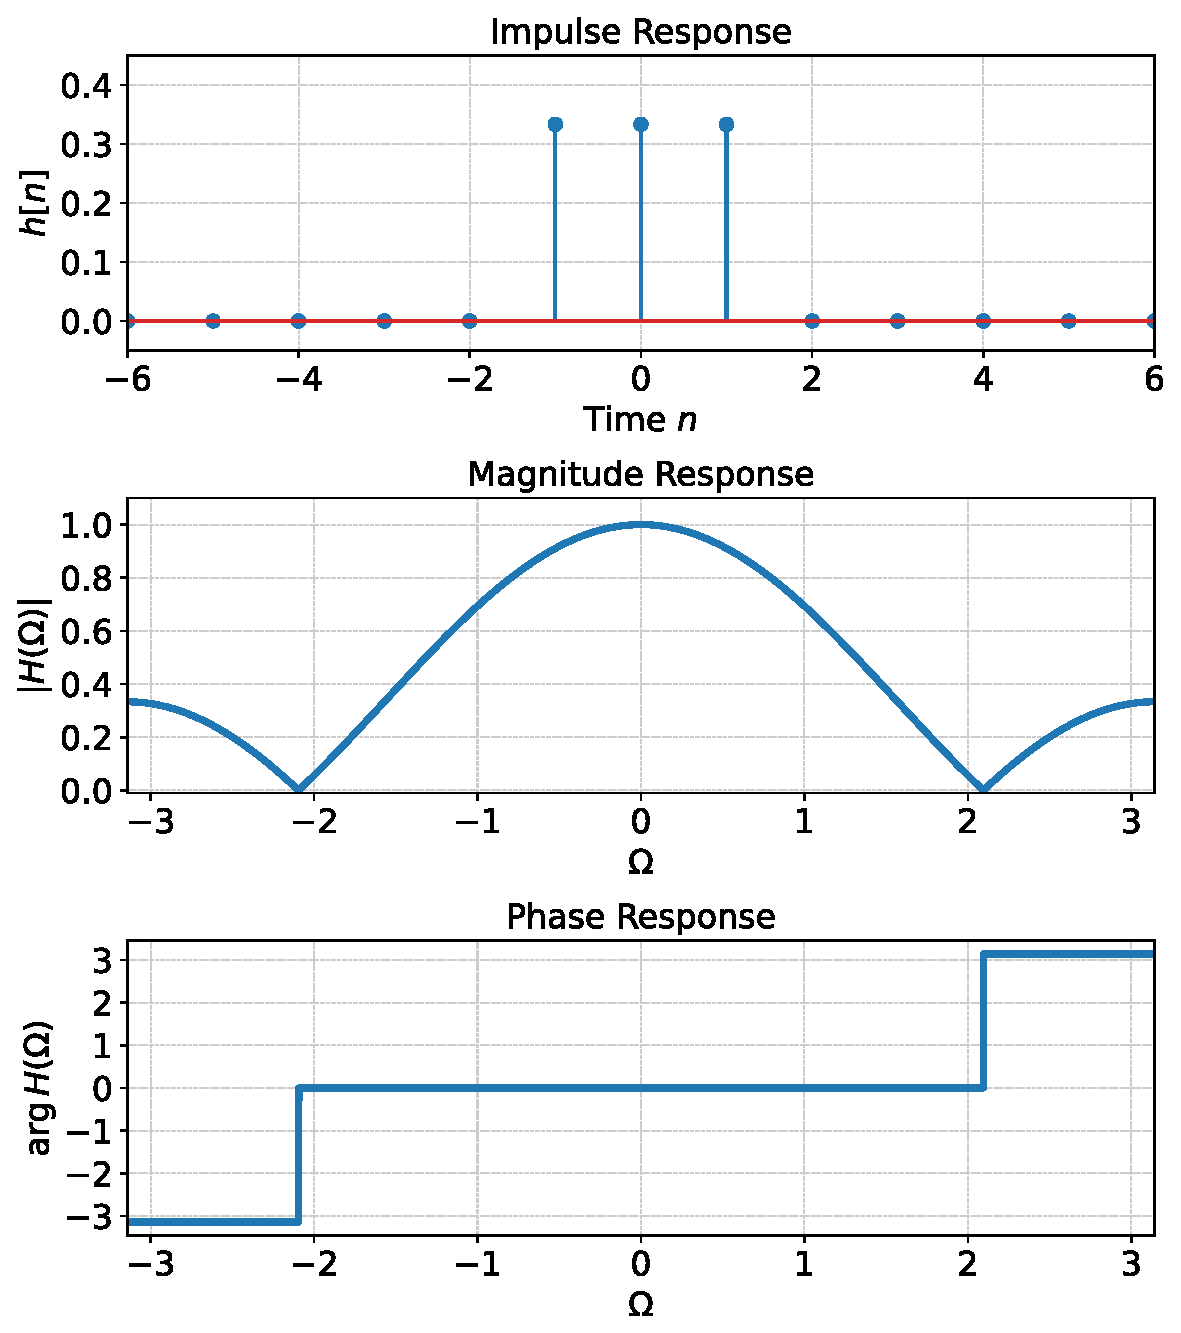
\includegraphics[width=0.4\textwidth]{img/movavg.eps}
  \end{figure}
  \end{center}
\end{frame}


\begin{frame}[t]{Response of an LTI system to a complex exponential}
\[ x[n] \rightarrow X\lp \Omega \rp \longrightarrow H\lp \Omega \rp X\lp \Omega \rp \rightarrow y[n]\]
\[ \big \vert Y\lp \Omega \rp \big \vert = \big \vert H\lp \Omega \rp\big \vert \big \vert X\lp \Omega \rp\big \vert \]
\[ \arg  \, \{ Y\lp \Omega \rp \} = \arg \{ H\lp \Omega \rp \} + \arg \{ X\lp \Omega \rp \} \]

\[ y[n] = \frac{1}{2\pi} \int_{-\pi}^{\pi} Y\lp \Omega \rp e^{j\Omega n} d\Omega \]
\end{frame}


% \begin{frame}[t]
%   \frametitle{Ideal filters}
%   \begin{center}
%   \begin{figure}
%   \centering
%   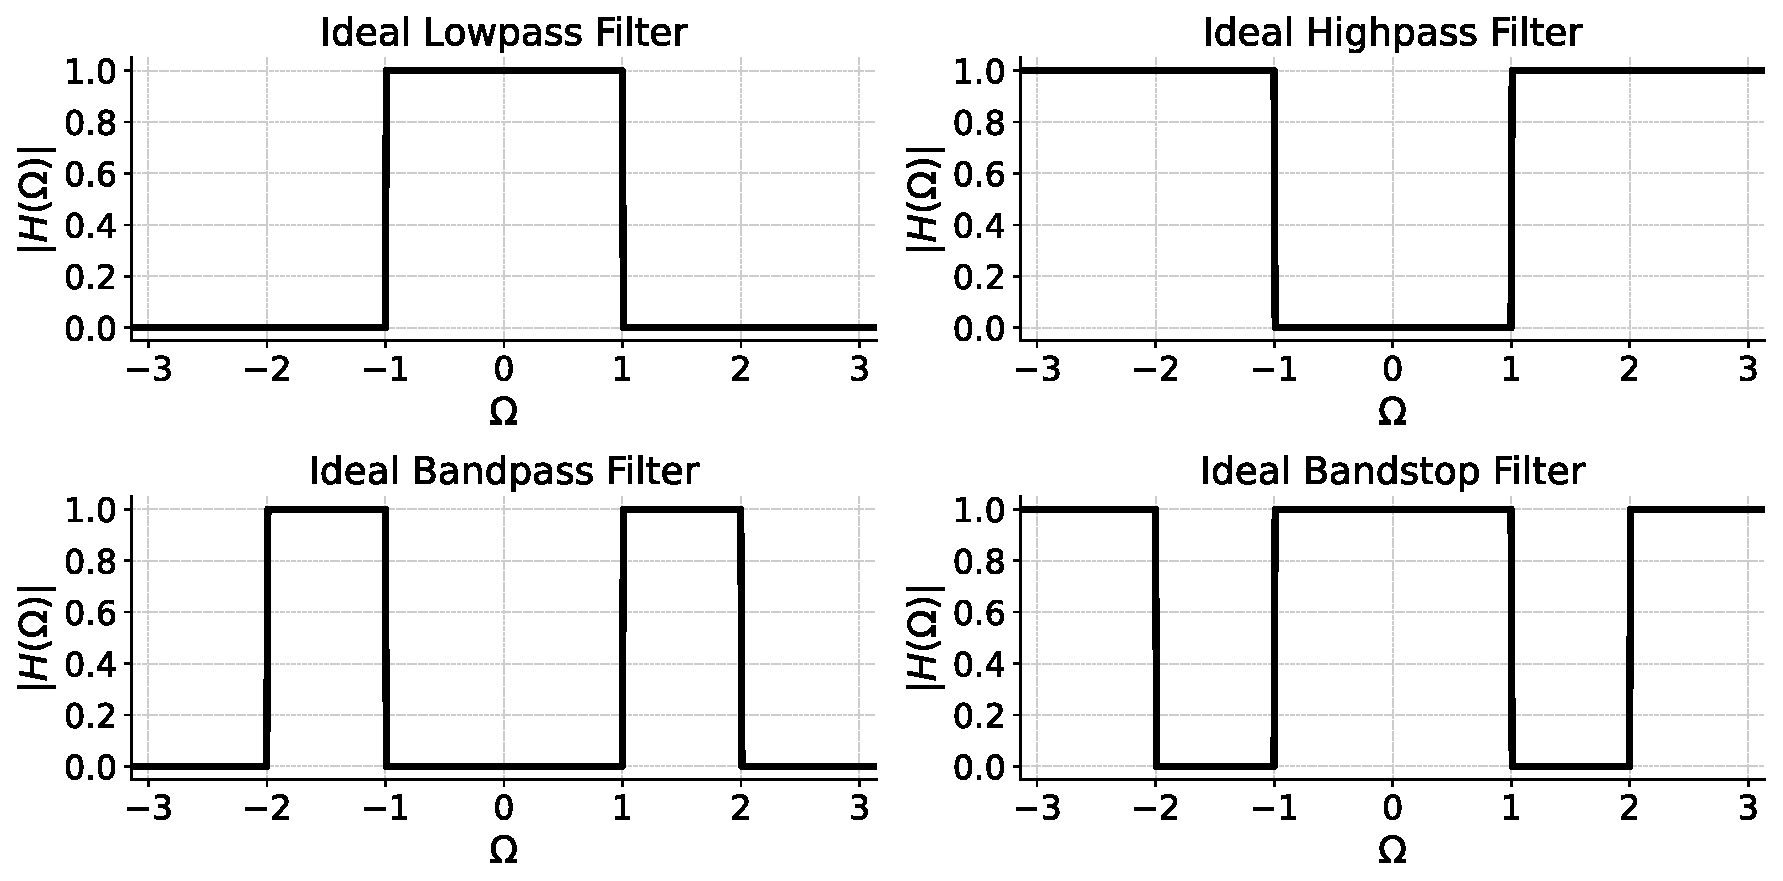
\includegraphics[width=0.9\textwidth]{img/idealfilt.eps}
%   \end{figure}
%   \end{center}
% \end{frame}

\end{document}